


\tikzset{every picture/.style={line width=0.75pt}} %set default line width to 0.75pt        

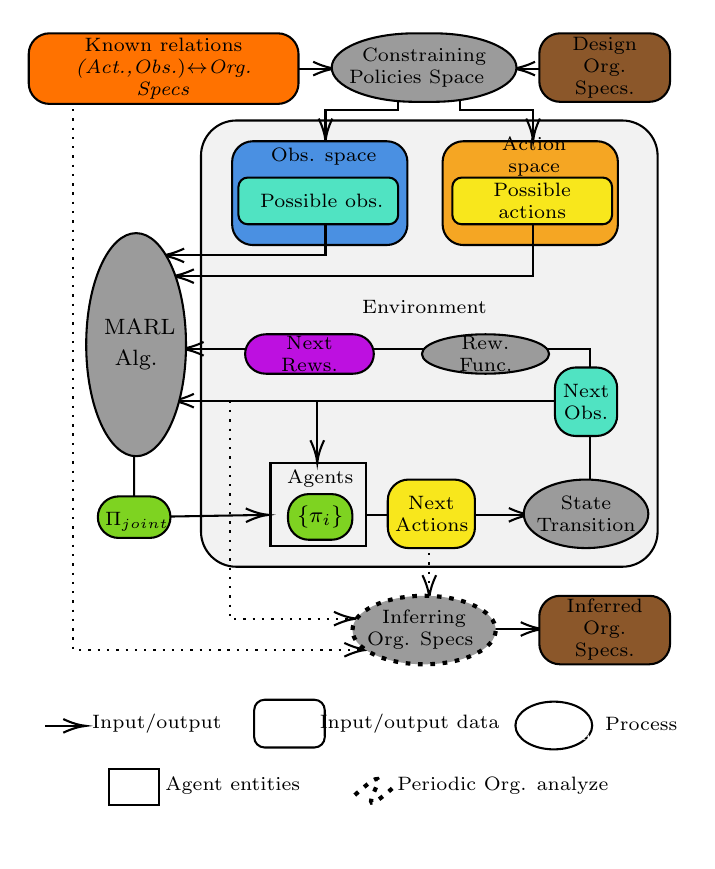
\begin{tikzpicture}[x=0.75pt,y=0.75pt,yscale=-1,xscale=1]
%uncomment if require: \path (0,1886); %set diagram left start at 0, and has height of 1886

%Shape: Rectangle [id:dp401980378305848] 
\draw  [fill={rgb, 255:red, 242; green, 242; blue, 242 }  ,fill opacity=1 ] (110,1267) .. controls (110,1257.61) and (117.61,1250) .. (127,1250) -- (313,1250) .. controls (322.39,1250) and (330,1257.61) .. (330,1267) -- (330,1448) .. controls (330,1457.39) and (322.39,1465) .. (313,1465) -- (127,1465) .. controls (117.61,1465) and (110,1457.39) .. (110,1448) -- cycle ;
%Straight Lines [id:da3175929748716908] 
\draw    (140.56,1440.03) -- (77.8,1441.11) -- (77.8,1396.11) ;
\draw [shift={(142.56,1440)}, rotate = 179.02] [color={rgb, 255:red, 0; green, 0; blue, 0 }  ][line width=0.75]    (10.93,-3.29) .. controls (6.95,-1.4) and (3.31,-0.3) .. (0,0) .. controls (3.31,0.3) and (6.95,1.4) .. (10.93,3.29)   ;
%Straight Lines [id:da6945547491407538] 
\draw    (297.41,1425) -- (297.41,1360) -- (102.33,1360) ;
\draw [shift={(100.33,1360)}, rotate = 360] [color={rgb, 255:red, 0; green, 0; blue, 0 }  ][line width=0.75]    (10.93,-3.29) .. controls (6.95,-1.4) and (3.31,-0.3) .. (0,0) .. controls (3.31,0.3) and (6.95,1.4) .. (10.93,3.29)   ;
%Straight Lines [id:da9008612661222812] 
\draw    (267.26,1440) -- (189.48,1440) ;
\draw [shift={(269.26,1440)}, rotate = 180] [color={rgb, 255:red, 0; green, 0; blue, 0 }  ][line width=0.75]    (10.93,-3.29) .. controls (6.95,-1.4) and (3.31,-0.3) .. (0,0) .. controls (3.31,0.3) and (6.95,1.4) .. (10.93,3.29)   ;
%Straight Lines [id:da7449421779677099] 
\draw    (166.02,1385) -- (166.02,1394.54) -- (166.02,1413) ;
\draw [shift={(166.02,1415)}, rotate = 270] [color={rgb, 255:red, 0; green, 0; blue, 0 }  ][line width=0.75]    (10.93,-3.29) .. controls (6.95,-1.4) and (3.31,-0.3) .. (0,0) .. controls (3.31,0.3) and (6.95,1.4) .. (10.93,3.29)   ;
%Rounded Rect [id:dp5816576242467624] 
\draw  [fill={rgb, 255:red, 245; green, 166; blue, 35 }  ,fill opacity=1 ] (226.41,1270) .. controls (226.41,1264.48) and (230.89,1260) .. (236.41,1260) -- (300.87,1260) .. controls (306.4,1260) and (310.87,1264.48) .. (310.87,1270) -- (310.87,1300) .. controls (310.87,1305.52) and (306.4,1310) .. (300.87,1310) -- (236.41,1310) .. controls (230.89,1310) and (226.41,1305.52) .. (226.41,1300) -- cycle ;
%Rounded Rect [id:dp9529058754609632] 
\draw  [fill={rgb, 255:red, 248; green, 231; blue, 28 }  ,fill opacity=1 ] (231.1,1282) .. controls (231.1,1279.51) and (233.12,1277.5) .. (235.6,1277.5) -- (303.56,1277.5) .. controls (306.04,1277.5) and (308.06,1279.51) .. (308.06,1282) -- (308.06,1295.5) .. controls (308.06,1297.99) and (306.04,1300) .. (303.56,1300) -- (235.6,1300) .. controls (233.12,1300) and (231.1,1297.99) .. (231.1,1295.5) -- cycle ;
%Straight Lines [id:da451152930226852] 
\draw    (283.33,1385) -- (97.63,1385) ;
\draw [shift={(95.63,1385)}, rotate = 360] [color={rgb, 255:red, 0; green, 0; blue, 0 }  ][line width=0.75]    (10.93,-3.29) .. controls (6.95,-1.4) and (3.31,-0.3) .. (0,0) .. controls (3.31,0.3) and (6.95,1.4) .. (10.93,3.29)   ;
%Straight Lines [id:da9734446377197741] 
\draw  [dash pattern={on 0.84pt off 2.51pt}]  (123.79,1385) -- (123.79,1490) -- (183,1490) ;
\draw [shift={(185,1490)}, rotate = 180] [color={rgb, 255:red, 0; green, 0; blue, 0 }  ][line width=0.75]    (10.93,-3.29) .. controls (6.95,-1.4) and (3.31,-0.3) .. (0,0) .. controls (3.31,0.3) and (6.95,1.4) .. (10.93,3.29)   ;
%Straight Lines [id:da9129668939660789] 
\draw    (164.39,1225) -- (125,1225) -- (173,1225) ;
\draw [shift={(175,1225)}, rotate = 180] [color={rgb, 255:red, 0; green, 0; blue, 0 }  ][line width=0.75]    (10.93,-3.29) .. controls (6.95,-1.4) and (3.31,-0.3) .. (0,0) .. controls (3.31,0.3) and (6.95,1.4) .. (10.93,3.29)   ;
%Straight Lines [id:da3918848581834071] 
\draw  [dash pattern={on 0.84pt off 2.51pt}]  (48.3,1240) -- (48.3,1505) -- (188,1505) ;
\draw [shift={(190,1505)}, rotate = 180] [color={rgb, 255:red, 0; green, 0; blue, 0 }  ][line width=0.75]    (10.93,-3.29) .. controls (6.95,-1.4) and (3.31,-0.3) .. (0,0) .. controls (3.31,0.3) and (6.95,1.4) .. (10.93,3.29)   ;
%Straight Lines [id:da46383821746892684] 
\draw    (285.34,1225) -- (262,1225) ;
\draw [shift={(260,1225)}, rotate = 360] [color={rgb, 255:red, 0; green, 0; blue, 0 }  ][line width=0.75]    (10.93,-3.29) .. controls (6.95,-1.4) and (3.31,-0.3) .. (0,0) .. controls (3.31,0.3) and (6.95,1.4) .. (10.93,3.29)   ;
%Straight Lines [id:da8847181725148201] 
\draw    (251.2,1495) -- (273,1495) ;
\draw [shift={(275,1495)}, rotate = 180] [color={rgb, 255:red, 0; green, 0; blue, 0 }  ][line width=0.75]    (10.93,-3.29) .. controls (6.95,-1.4) and (3.31,-0.3) .. (0,0) .. controls (3.31,0.3) and (6.95,1.4) .. (10.93,3.29)   ;
%Shape: Rectangle [id:dp08035475030295403] 
\draw   (143.5,1415) -- (189.48,1415) -- (189.48,1455) -- (143.5,1455) -- cycle ;
%Straight Lines [id:da24098465376222578] 
\draw    (205,1240) -- (205,1245) -- (170,1245) -- (170,1258) ;
\draw [shift={(170,1260)}, rotate = 270] [color={rgb, 255:red, 0; green, 0; blue, 0 }  ][line width=0.75]    (10.93,-3.29) .. controls (6.95,-1.4) and (3.31,-0.3) .. (0,0) .. controls (3.31,0.3) and (6.95,1.4) .. (10.93,3.29)   ;
%Shape: Boxed Line [id:dp8352454731616787] 
\draw    (35,1541.67) -- (52.58,1541.67) ;
\draw [shift={(54.58,1541.67)}, rotate = 180] [color={rgb, 255:red, 0; green, 0; blue, 0 }  ][line width=0.75]    (10.93,-3.29) .. controls (6.95,-1.4) and (3.31,-0.3) .. (0,0) .. controls (3.31,0.3) and (6.95,1.4) .. (10.93,3.29)   ;
%Shape: Rectangle [id:dp6328669951136969] 
\draw   (65.57,1562.23) -- (89.65,1562.23) -- (89.65,1580) -- (65.57,1580) -- cycle ;
%Curve Lines [id:da763384068727073] 
\draw [line width=1.5]  [dash pattern={on 1.69pt off 2.76pt}]  (184.12,1574.99) .. controls (212.34,1549.77) and (174.94,1596.12) .. (203.15,1570.9) ;

%Rounded Rect [id:dp3278199732714804] 
\draw  [fill={rgb, 255:red, 74; green, 144; blue, 226 }  ,fill opacity=1 ] (125,1270) .. controls (125,1264.48) and (129.48,1260) .. (135,1260) -- (199.47,1260) .. controls (204.99,1260) and (209.47,1264.48) .. (209.47,1270) -- (209.47,1300) .. controls (209.47,1305.52) and (204.99,1310) .. (199.47,1310) -- (135,1310) .. controls (129.48,1310) and (125,1305.52) .. (125,1300) -- cycle ;
%Rounded Rect [id:dp24054971346627085] 
\draw  [fill={rgb, 255:red, 80; green, 227; blue, 194 }  ,fill opacity=1 ] (128.04,1282) .. controls (128.04,1279.51) and (130.06,1277.5) .. (132.54,1277.5) -- (200.5,1277.5) .. controls (202.99,1277.5) and (205,1279.51) .. (205,1282) -- (205,1295.5) .. controls (205,1297.99) and (202.99,1300) .. (200.5,1300) -- (132.54,1300) .. controls (130.06,1300) and (128.04,1297.99) .. (128.04,1295.5) -- cycle ;
%Straight Lines [id:da12662032901914455] 
\draw    (92.94,1315) -- (170,1315) -- (170,1300) ;
\draw [shift={(90.94,1315)}, rotate = 0] [color={rgb, 255:red, 0; green, 0; blue, 0 }  ][line width=0.75]    (10.93,-3.29) .. controls (6.95,-1.4) and (3.31,-0.3) .. (0,0) .. controls (3.31,0.3) and (6.95,1.4) .. (10.93,3.29)   ;
%Straight Lines [id:da6903330894551778] 
\draw    (270,1300) -- (270,1325) -- (97.63,1325) ;
\draw [shift={(95.63,1325)}, rotate = 360] [color={rgb, 255:red, 0; green, 0; blue, 0 }  ][line width=0.75]    (10.93,-3.29) .. controls (6.95,-1.4) and (3.31,-0.3) .. (0,0) .. controls (3.31,0.3) and (6.95,1.4) .. (10.93,3.29)   ;
%Straight Lines [id:da5241788732296702] 
\draw  [dash pattern={on 0.84pt off 2.51pt}]  (220,1445) -- (220,1478) ;
\draw [shift={(220,1480)}, rotate = 270] [color={rgb, 255:red, 0; green, 0; blue, 0 }  ][line width=0.75]    (10.93,-3.29) .. controls (6.95,-1.4) and (3.31,-0.3) .. (0,0) .. controls (3.31,0.3) and (6.95,1.4) .. (10.93,3.29)   ;
%Shape: Boxed Line [id:dp4508196331907264] 
\draw    (235,1240) -- (235,1245) -- (270,1245) -- (270,1258) ;
\draw [shift={(270,1260)}, rotate = 270] [color={rgb, 255:red, 0; green, 0; blue, 0 }  ][line width=0.75]    (10.93,-3.29) .. controls (6.95,-1.4) and (3.31,-0.3) .. (0,0) .. controls (3.31,0.3) and (6.95,1.4) .. (10.93,3.29)   ;


% Text Node
\draw (168.17,1288.75) node  [font=\scriptsize] [align=left] {\begin{minipage}[lt]{45.19pt}\setlength\topsep{0pt}
\begin{center}
Possible obs.
\end{center}

\end{minipage}};
% Text Node
\draw (169.11,1267.5) node  [font=\scriptsize] [align=left] {\begin{minipage}[lt]{38.85pt}\setlength\topsep{0pt}
\begin{center}
Obs. space
\end{center}

\end{minipage}};
% Text Node
\draw  [fill={rgb, 255:red, 139; green, 87; blue, 42 }  ,fill opacity=1 ]  (273,1489) .. controls (273,1483.48) and (277.48,1479) .. (283,1479) -- (326,1479) .. controls (331.52,1479) and (336,1483.48) .. (336,1489) -- (336,1502) .. controls (336,1507.52) and (331.52,1512) .. (326,1512) -- (283,1512) .. controls (277.48,1512) and (273,1507.52) .. (273,1502) -- cycle  ;
\draw (304.5,1495.5) node  [font=\scriptsize] [align=left] {\begin{minipage}[lt]{40.43pt}\setlength\topsep{0pt}
\begin{center}
Inferred\\Org. Specs.
\end{center}

\end{minipage}};
% Text Node
\draw  [color={rgb, 255:red, 0; green, 0; blue, 0 }  ,draw opacity=1 ][fill={rgb, 255:red, 155; green, 155; blue, 155 }  ,fill opacity=1 ][dash pattern={on 1.69pt off 2.76pt}][line width=1.5]   (183,1495.5) .. controls (183,1486.39) and (198.45,1479) .. (217.5,1479) .. controls (236.55,1479) and (252,1486.39) .. (252,1495.5) .. controls (252,1504.61) and (236.55,1512) .. (217.5,1512) .. controls (198.45,1512) and (183,1504.61) .. (183,1495.5) -- cycle  ;
\draw (217.5,1495.5) node  [font=\scriptsize] [align=left] {\begin{minipage}[lt]{44.39pt}\setlength\topsep{0pt}
\begin{center}
Inferring\\Org. Specs \ \ 
\end{center}

\end{minipage}};
% Text Node
\draw  [fill={rgb, 255:red, 248; green, 231; blue, 28 }  ,fill opacity=1 ]  (200,1433) .. controls (200,1427.48) and (204.48,1423) .. (210,1423) -- (232,1423) .. controls (237.52,1423) and (242,1427.48) .. (242,1433) -- (242,1446) .. controls (242,1451.52) and (237.52,1456) .. (232,1456) -- (210,1456) .. controls (204.48,1456) and (200,1451.52) .. (200,1446) -- cycle  ;
\draw (221,1439.5) node  [font=\scriptsize] [align=left] {\begin{minipage}[lt]{26.14pt}\setlength\topsep{0pt}
\begin{center}
Next\\Actions
\end{center}

\end{minipage}};
% Text Node
\draw  [fill={rgb, 255:red, 126; green, 211; blue, 33 }  ,fill opacity=1 ]  (151.93,1440) .. controls (151.93,1434.48) and (156.41,1430) .. (161.93,1430) -- (172.93,1430) .. controls (178.45,1430) and (182.93,1434.48) .. (182.93,1440) -- (182.93,1442) .. controls (182.93,1447.52) and (178.45,1452) .. (172.93,1452) -- (161.93,1452) .. controls (156.41,1452) and (151.93,1447.52) .. (151.93,1442) -- cycle  ;
\draw (167.43,1441) node  [font=\footnotesize] [align=left] {\begin{minipage}[lt]{18.45pt}\setlength\topsep{0pt}
\begin{center}
$\displaystyle \{\pi _{i}\}$
\end{center}

\end{minipage}};
% Text Node
\draw (167.43,1422.5) node  [font=\scriptsize] [align=left] {\begin{minipage}[lt]{24.96pt}\setlength\topsep{0pt}
\begin{center}
Agents
\end{center}

\end{minipage}};
% Text Node
\draw  [fill={rgb, 255:red, 80; green, 227; blue, 194 }  ,fill opacity=1 ]  (280.53,1379) .. controls (280.53,1373.48) and (285.01,1369) .. (290.53,1369) -- (300.53,1369) .. controls (306.06,1369) and (310.53,1373.48) .. (310.53,1379) -- (310.53,1392) .. controls (310.53,1397.52) and (306.06,1402) .. (300.53,1402) -- (290.53,1402) .. controls (285.01,1402) and (280.53,1397.52) .. (280.53,1392) -- cycle  ;
\draw (295.53,1385.5) node  [font=\scriptsize] [align=left] {\begin{minipage}[lt]{17.81pt}\setlength\topsep{0pt}
\begin{center}
Next\\Obs.
\end{center}

\end{minipage}};
% Text Node
\draw  [fill={rgb, 255:red, 155; green, 155; blue, 155 }  ,fill opacity=1 ]  (173,1224.5) .. controls (173,1215.39) and (190.91,1208) .. (213,1208) -- (222,1208) .. controls (244.09,1208) and (262,1215.39) .. (262,1224.5) .. controls (262,1233.61) and (244.09,1241) .. (222,1241) -- (213,1241) .. controls (190.91,1241) and (173,1233.61) .. (173,1224.5) -- cycle  ;
\draw (217.5,1224.5) node  [font=\scriptsize] [align=left] {\begin{minipage}[lt]{57.49pt}\setlength\topsep{0pt}
\begin{center}
Constraining\\Policies Space \ \ \ 
\end{center}

\end{minipage}};
% Text Node
\draw  [fill={rgb, 255:red, 255; green, 114; blue, 0 }  ,fill opacity=1 ]  (27,1218) .. controls (27,1212.48) and (31.48,1208) .. (37,1208) -- (147,1208) .. controls (152.52,1208) and (157,1212.48) .. (157,1218) -- (157,1232) .. controls (157,1237.52) and (152.52,1242) .. (147,1242) -- (37,1242) .. controls (31.48,1242) and (27,1237.52) .. (27,1232) -- cycle  ;
\draw (92,1225) node  [font=\scriptsize] [align=left] {\begin{minipage}[lt]{85.61pt}\setlength\topsep{0pt}
\begin{center}
Known relations\\\textit{(Act.,Obs.})$\displaystyle \leftrightarrow $\textit{Org. Specs}
\end{center}

\end{minipage}};
% Text Node
\draw  [fill={rgb, 255:red, 189; green, 16; blue, 224 }  ,fill opacity=1 ]  (131.27,1362.5) .. controls (131.27,1357.25) and (135.74,1353) .. (141.27,1353) -- (183.27,1353) .. controls (188.79,1353) and (193.27,1357.25) .. (193.27,1362.5) .. controls (193.27,1367.75) and (188.79,1372) .. (183.27,1372) -- (141.27,1372) .. controls (135.74,1372) and (131.27,1367.75) .. (131.27,1362.5) -- cycle  ;
\draw (162.27,1362.5) node  [font=\scriptsize] [align=left] {\begin{minipage}[lt]{39.23pt}\setlength\topsep{0pt}
\begin{center}
Next Rews.
\end{center}

\end{minipage}};
% Text Node
\draw  [fill={rgb, 255:red, 155; green, 155; blue, 155 }  ,fill opacity=1 ]  (265.53,1439.5) .. controls (265.53,1430.39) and (278.97,1423) .. (295.53,1423) .. controls (312.1,1423) and (325.53,1430.39) .. (325.53,1439.5) .. controls (325.53,1448.61) and (312.1,1456) .. (295.53,1456) .. controls (278.97,1456) and (265.53,1448.61) .. (265.53,1439.5) -- cycle  ;
\draw (295.53,1439.5) node  [font=\scriptsize] [align=left] {\begin{minipage}[lt]{37.77pt}\setlength\topsep{0pt}
\begin{center}
State\\Transition \ 
\end{center}

\end{minipage}};
% Text Node
\draw  [fill={rgb, 255:red, 126; green, 211; blue, 33 }  ,fill opacity=1 ]  (60.3,1441.11) .. controls (60.3,1435.58) and (64.78,1431.11) .. (70.3,1431.11) -- (85.3,1431.11) .. controls (90.82,1431.11) and (95.3,1435.58) .. (95.3,1441.11) .. controls (95.3,1446.63) and (90.82,1451.11) .. (85.3,1451.11) -- (70.3,1451.11) .. controls (64.78,1451.11) and (60.3,1446.63) .. (60.3,1441.11) -- cycle  ;
\draw (77.8,1441.11) node  [font=\scriptsize] [align=left] {\begin{minipage}[lt]{20.95pt}\setlength\topsep{0pt}
\begin{center}
$\displaystyle \Pi _{joint}$
\end{center}

\end{minipage}};
% Text Node
\draw  [fill={rgb, 255:red, 155; green, 155; blue, 155 }  ,fill opacity=1 ]  (78.74, 1358) circle [x radius= 24.04, y radius= 53.74]   ;
\draw (78.74,1358) node  [font=\small] [align=left] {\begin{minipage}[lt]{23.12pt}\setlength\topsep{0pt}
\begin{center}
\phantom{x}\\{\footnotesize MARL}\\{\footnotesize Alg.}\\\phantom{x}
\end{center}

\end{minipage}};
% Text Node
\draw (269.58,1288.75) node  [font=\scriptsize] [align=left] {\begin{minipage}[lt]{54.32pt}\setlength\topsep{0pt}
\begin{center}
Possible actions
\end{center}

\end{minipage}};
% Text Node
\draw (270.52,1267.5) node  [font=\scriptsize] [align=left] {\begin{minipage}[lt]{43.61pt}\setlength\topsep{0pt}
\begin{center}
Action space
\end{center}

\end{minipage}};
% Text Node
\draw (216.23,1337.5) node  [font=\scriptsize] [align=left] {\begin{minipage}[lt]{42.81pt}\setlength\topsep{0pt}
\begin{center}
Environment
\end{center}

\end{minipage}};
% Text Node
\draw  [fill={rgb, 255:red, 155; green, 155; blue, 155 }  ,fill opacity=1 ]  (216.45,1362.5) .. controls (216.45,1357.25) and (230.16,1353) .. (247.08,1353) .. controls (264,1353) and (277.71,1357.25) .. (277.71,1362.5) .. controls (277.71,1367.75) and (264,1372) .. (247.08,1372) .. controls (230.16,1372) and (216.45,1367.75) .. (216.45,1362.5) -- cycle  ;
\draw (247.08,1362.5) node  [font=\scriptsize,xslant=-0.02] [align=left] {\begin{minipage}[lt]{38.44pt}\setlength\topsep{0pt}
\begin{center}
Rew. Func.
\end{center}

\end{minipage}};
% Text Node
\draw  [fill={rgb, 255:red, 139; green, 87; blue, 42 }  ,fill opacity=1 ]  (273,1218) .. controls (273,1212.48) and (277.48,1208) .. (283,1208) -- (326,1208) .. controls (331.52,1208) and (336,1212.48) .. (336,1218) -- (336,1231) .. controls (336,1236.52) and (331.52,1241) .. (326,1241) -- (283,1241) .. controls (277.48,1241) and (273,1236.52) .. (273,1231) -- cycle  ;
\draw (304.5,1224.5) node  [font=\scriptsize] [align=left] {\begin{minipage}[lt]{40.43pt}\setlength\topsep{0pt}
\begin{center}
Design\\Org. Specs.
\end{center}

\end{minipage}};
% Text Node
\draw (322.13,1540.49) node  [font=\small] [align=left] {{\scriptsize Process}};
% Text Node
\draw    (261.49,1541.49) .. controls (261.49,1535.13) and (269.77,1529.99) .. (279.99,1529.99) .. controls (290.21,1529.99) and (298.49,1535.13) .. (298.49,1541.49) .. controls (298.49,1547.84) and (290.21,1552.99) .. (279.99,1552.99) .. controls (269.77,1552.99) and (261.49,1547.84) .. (261.49,1541.49) -- cycle  ;
\draw (279.99,1541.49) node  [font=\small] [align=left] {\begin{minipage}[lt]{22.12pt}\setlength\topsep{0pt}
\begin{center}
\textcolor[rgb]{1,1,1}{{\tiny aassssaa}}
\end{center}

\end{minipage}};
% Text Node
\draw (88.72,1540.49) node  [font=\small] [align=left] {{\scriptsize Input/output}};
% Text Node
\draw (210.52,1540.49) node  [font=\small] [align=left] {{\scriptsize Input/output data}};
% Text Node
\draw    (135.63,1534.08) .. controls (135.63,1531.32) and (137.87,1529.08) .. (140.63,1529.08) -- (164.63,1529.08) .. controls (167.39,1529.08) and (169.63,1531.32) .. (169.63,1534.08) -- (169.63,1547.08) .. controls (169.63,1549.84) and (167.39,1552.08) .. (164.63,1552.08) -- (140.63,1552.08) .. controls (137.87,1552.08) and (135.63,1549.84) .. (135.63,1547.08) -- cycle  ;
\draw (152.63,1540.58) node  [font=\small] [align=left] {\begin{minipage}[lt]{20.08pt}\setlength\topsep{0pt}
\begin{center}
\textcolor[rgb]{1,1,1}{{\tiny assaaaa}}
\end{center}

\end{minipage}};
% Text Node
\draw (255.44,1570.49) node  [font=\small] [align=left] {{\scriptsize Periodic Org. analyze}};
% Text Node
\draw (125.31,1570.49) node  [font=\small] [align=left] {{\scriptsize Agent entities}};


\end{tikzpicture}